\section{Definitions}                    % notation, frames and models used in the report
\label{sec:definitions}                  % \secref{sec:definitions}

The scan-merging method implemented in this project is the one proposed by
\citet{breux2020elevation} for a vehicle carrying the same pair of perpendicular sonars. This
section fixes the notation, frames and models of that work, adapted to the NavScoot~2, and
used in the rest of the report.

% ------------------------------------------------------------------------------
\subsection{Notation}                    % general conventions
\label{sec:def_notation}                 % \secref{sec:def_notation}

\begin{itemize}                          % one convention per item
  \item Vectors are written in bold lower case ($\mathbf{x}$) and matrices in upper case
        ($\mathbf{M}$). $\mathbf{x}|_{\{R\}}$ denotes a vector expressed in the frame $\{R\}$.
  \item $X \sim q(\lambda)$ means that the random variable $X$ follows the law of probability
        density function (pdf) $q$ with parameters $\lambda$; $\mathcal{N}(\boldsymbol{\mu},
        \boldsymbol{\Sigma})$ is the Gaussian law of mean $\boldsymbol{\mu}$ and covariance
        $\boldsymbol{\Sigma}$. $\hat{X}$ denotes an estimate of $X$.
  \item $SE(3)$ is the group of rigid transformations of space. A pose is stored as a position and a
        unit quaternion $\mathbf{q}$, whose rotation matrix is $\mathbf{R}(\mathbf{q})$, or as the
        equivalent $4\times4$ homogeneous matrix $\mathbf{T} = \begin{bmatrix} \mathbf{R} &
        \boldsymbol{\tau} \\ \mathbf{0} & 1 \end{bmatrix}$.
  \item $SE(3)$ is a Lie group; its Lie algebra $\mathfrak{se}(3)$ holds the infinitesimal motions,
        written as 6-vectors $\boldsymbol{\xi} = [\mathbf{v}^T\ \boldsymbol{\omega}^T]^T$ with a
        translational part $\mathbf{v}$ and a rotational part $\boldsymbol{\omega}$. The logarithm
        map $\log : SE(3) \to \mathfrak{se}(3)$ returns the motion that leads from the identity to a
        given transformation. $T_{\mathbf{A}}SE(3)$ is the tangent space of $SE(3)$ at
        $\mathbf{A}$ and $\langle \cdot, \cdot \rangle_{\mathbf{A}}$ an inner product on it; $e$ is
        the identity element.
  \item Orientations can also be given by Euler angles $[\psi\ \chi\ \phi]^T$ (yaw, pitch, roll),
        with rotation matrix $\mathbf{R}(\psi, \chi, \phi)$; these angles are written with a
        $\delta$ when they are increments, to distinguish them from the sonar angles $\psi^h$,
        $\psi^v$. $[\boldsymbol{\omega}]_\times$ is the skew-symmetric matrix such that
        $[\boldsymbol{\omega}]_\times \mathbf{x} = \boldsymbol{\omega} \times \mathbf{x}$.
  \item $\oplus$ (resp.\ $\ominus$) is the composition (resp.\ inverse composition) of poses and
        points \citep{blanco2010tutorial}: if $\boldsymbol{\eta}$ is the pose of a frame and
        $\mathbf{x}$ a point expressed in that frame, $\boldsymbol{\eta} \oplus \mathbf{x}$ is the same
        point expressed in the frame in which $\boldsymbol{\eta}$ is given. Conversely,
        $\mathbf{x} \ominus \boldsymbol{\eta}$ expresses in the frame of pose $\boldsymbol{\eta}$ a
        point $\mathbf{x}$ given in the reference frame.
\end{itemize}

% ------------------------------------------------------------------------------
\subsection{Frames and poses}            % where everything is expressed
\label{sec:def_frames}                   % \secref{sec:def_frames}

Four frames are used (Figure~\ref{fig:def_frames}a): the fixed world frame $\{0\}$, the body frame
$\{B\}$ attached to the vehicle, and the frames $\{S_H\}$ and $\{S_V\}$ attached to the horizontal
and vertical sonar heads. With these frames:
\begin{itemize}                          % pose vectors
  \item $\boldsymbol{\tau}$ ($3\times1$) and $\mathbf{q}$ ($4\times1$) are the position and attitude of
        $\{B\}$ in $\{0\}$, and $\boldsymbol{\eta} = [\boldsymbol{\tau}^T\ \mathbf{q}^T]^T$ ($7\times1$)
        is the \emph{pose} of the vehicle;
  \item $\mathbf{p}_H = [\boldsymbol{\tau}_H^T\ \mathbf{q}_H^T]^T$ and
        $\mathbf{p}_V = [\boldsymbol{\tau}_V^T\ \mathbf{q}_V^T]^T$ are the fixed poses of $\{S_H\}$ and
        $\{S_V\}$ in $\{B\}$, given by the mounting of the sonars on the NavScoot~2
        \citep{margaritis2025internship}.
\end{itemize}
The navigation sensors (DVL, IMU, depth sensor) provide by dead reckoning a pose estimate at regular
times, assumed Gaussian, $\boldsymbol{\eta} \sim \mathcal{N}(\bar{\boldsymbol{\eta}},
\boldsymbol{\Sigma}_{\eta})$. The \emph{discretized trajectory} is the set of these poses,
$\mathcal{H} = \{\boldsymbol{\eta}_i\}$, $i \in \{1,\dots,n_r\}$.

% ------------------------------------------------------------------------------
\subsection{Sonar measurements}          % what one ping gives
\label{sec:def_measurements}             % \secref{sec:def_measurements}

Both sonars are mechanically scanned imaging sonars (MSIS): a head rotates step by step around one
axis and, at each step, emits a ping whose echoes give the range $\rho$ to the surrounding surface
$\Omega$. In the sonar frame, a point is described by its range $\rho$, its \emph{rotation angle}
$\psi$ (the angle of the head) and its \emph{elevation angle} $\theta$, defined as the oriented angle
between the $XY$-plane of the sonar frame and the measured ray. A beam has a vertical aperture
$\Theta$ and a horizontal aperture $\Psi$. On the NavScoot~2, the vertical sonar beam
(1--2$^\circ$) and the horizontal width of the horizontal sonar beam (2$^\circ$) are narrow, so
we take $\Psi_H = \Psi_V = \Theta_V = 0$. Only the vertical aperture of the horizontal sonar
is kept: $\Theta_H = [-b/2,\, b/2]$, with $b = 25^\circ$ for the Ping360.

\begin{itemize}                          % the two kinds of measurement
  \item \textbf{Vertical sonar.} A ping gives a single point,
        $\mathbf{m}^v_k = [\rho^v_k\ \ 0\ \ \psi^v_k]^T$ in $\{S_V\}$: its elevation is known and
        equal to zero.
  \item \textbf{Horizontal sonar.} Because of the aperture $\Theta_H$, a single ping can return
        $n$ echoes at different ranges $\rho^h_{ij}$ and \emph{unknown} elevation angles
        $\theta^h_{ij}$, all with the same rotation angle $\psi^h_i$
        (Figure~\ref{fig:def_frames}b). The $i$-th measurement is the $3\times n$ matrix
        $\mathbf{M}^h_i = [\mathbf{m}^h_{ij}]$, with
        $\mathbf{m}^h_{ij} = [\rho^h_{ij}\ \ \theta^h_{ij}\ \ \psi^h_i]^T$.
\end{itemize}

A \emph{complete scan} $\mathcal{S} = \{\mathcal{M}^h, \mathcal{M}^v\}$ gathers the measurements
$\mathcal{M}^h = \{\mathbf{M}^h_i\}$, $i \in \{1,\dots,n_h\}$, taken while the horizontal sonar
completes a full $360^\circ$ rotation, and the measurements
$\mathcal{M}^v = \{\mathbf{m}^v_k\}$, $k \in \{1,\dots,n_v\}$, of the vertical sonar over the same
time interval. Since the sonars and the navigation are not synchronized, the functions
$\sigma^h : \{1,\dots,n_h\} \to \{1,\dots,n_r\}$ and $\sigma^v : \{1,\dots,n_v\} \to
\{1,\dots,n_r\}$ return the index of the pose at which each measurement was taken. A measurement
is then placed in the world frame by
\begin{equation}                         % spherical sonar coordinates -> world point
  g^h(\rho, \theta, \psi, i) = \boldsymbol{\eta}_{\sigma^h(i)} \oplus \mathbf{p}_H \oplus
  \begin{bmatrix} \rho\cos\theta\cos\psi \\ \rho\cos\theta\sin\psi \\ \rho\sin\theta \end{bmatrix},
  \label{eq:def_gh}
\end{equation}
and $g^v$ is defined in the same way with $\sigma^v$ and $\mathbf{p}_V$. For a vertical
measurement every argument is known. For a horizontal one, $\theta$ is missing: estimating it is
the goal of scan merging and in general the goal of this project.

\begin{figure}[!htbp]                    % frames and the elevation ambiguity
  \centering
  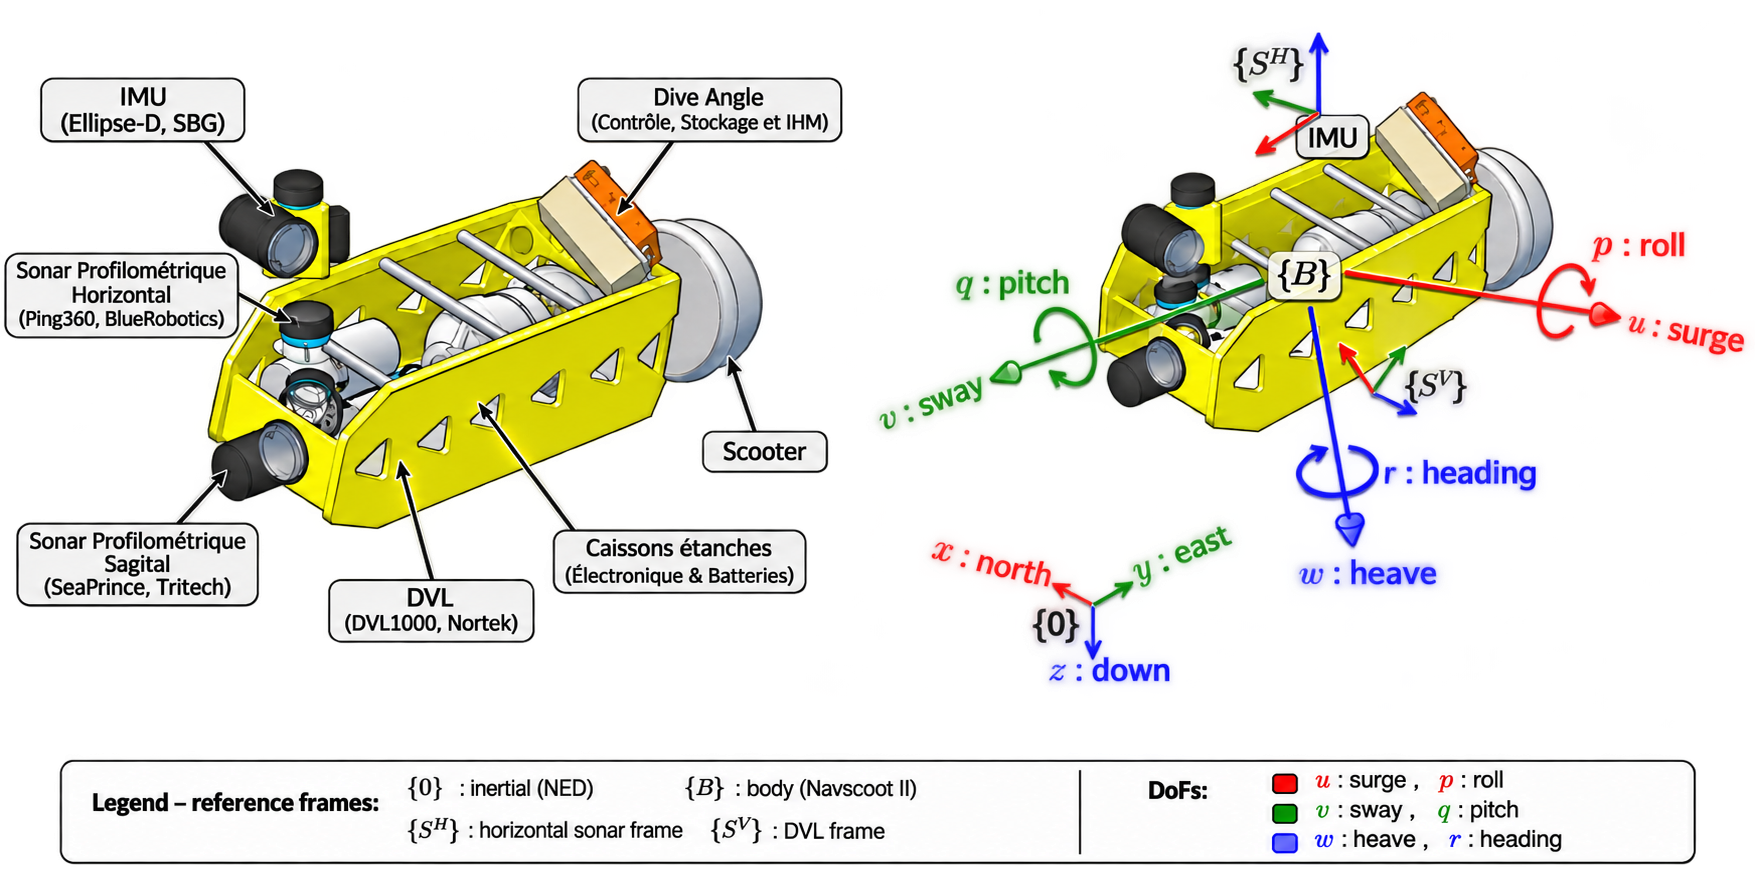
\includegraphics[width=0.8\linewidth, height=9cm, keepaspectratio]{figures/frames_used.png}\\[0.2em]
  {\small (a)}\\[0.8em]
  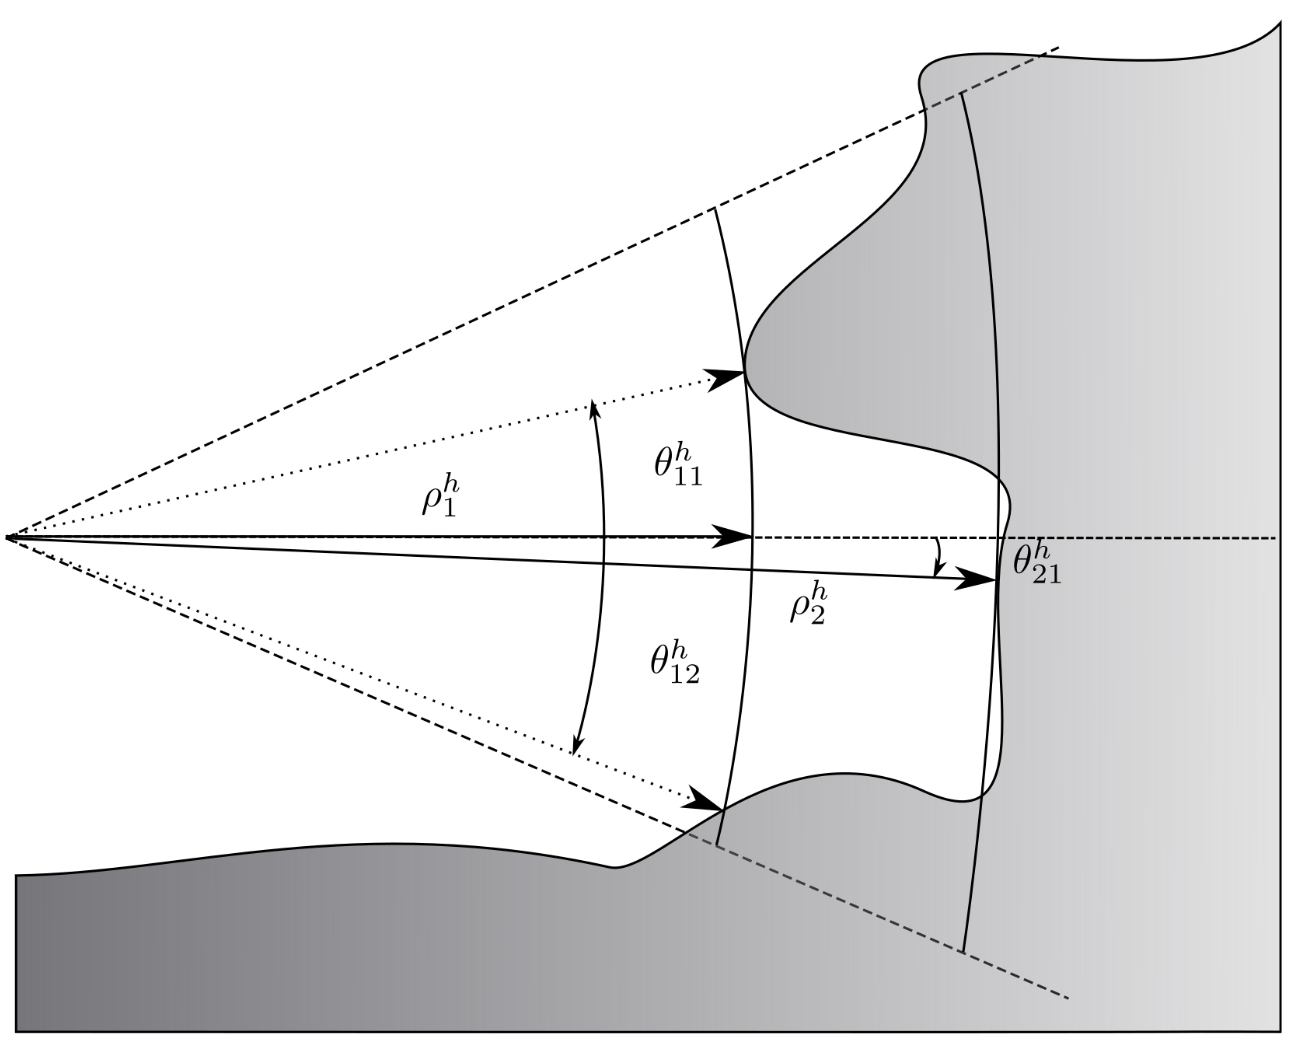
\includegraphics[width=0.8\linewidth, height=9cm, keepaspectratio]{figures/several_elevation_angles.png}\\[0.2em]
  {\small (b)}
  \caption{(a) Frames used in this report. (b) A single horizontal sonar ping can correspond to
           several 3D points, hence several elevation angles. Adapted from
           \citet{breux2020elevation}.}
  \label{fig:def_frames}
\end{figure}

% ------------------------------------------------------------------------------
\subsection{Gaussian process regression}  % the surface model
\label{sec:def_gp}                        % \secref{sec:def_gp}

A Gaussian process (GP) is a set of random variables of which every finite subset follows a joint
Gaussian law \citep{rasmussen2006gaussian}. A GP $f \sim \mathcal{GP}(f_p, K)$ is defined by a prior
mean function $f_p$ and a covariance function, or \emph{kernel}, $K(\mathbf{x}, \mathbf{x}')$, which
measures how similar the outputs at two inputs are expected to be. GP regression uses it as a
non-parametric model of an unknown function. Here it models the conduit surface seen by the
vertical sonar: the inputs are the curvilinear abscissa $s$ of the pose along the trajectory
(\secref{sec:msis_merging}) and the rotation angle $\psi^v$, and the output is the range,
\begin{equation}                         % observation model
  \rho^v = f(s, \psi^v) + e, \qquad e \sim \mathcal{N}(0, \sigma_n^2).
  \label{eq:def_gp_model}
\end{equation}
Given $N$ training inputs $\mathbf{X}$ with observed ranges $\mathbf{y}$, the prediction at a new input
$\mathbf{x}_*$ is Gaussian, $\rho_* \sim \mathcal{N}(\bar{\rho}_*, \sigma^2_{\rho_*})$, with
\begin{align}                            % GP posterior mean and variance
  \bar{\rho}_*      &= f_p(\mathbf{x}_*) + \mathbf{k}_*^T(\mathbf{K} + \sigma_n^2\mathbf{I})^{-1}
                       \big(\mathbf{y} - f_p(\mathbf{X})\big), \label{eq:def_gp_mean}\\
  \sigma^2_{\rho_*} &= K(\mathbf{x}_*, \mathbf{x}_*) - \mathbf{k}_*^T(\mathbf{K} +
                       \sigma_n^2\mathbf{I})^{-1}\mathbf{k}_*, \label{eq:def_gp_var}
\end{align}
where $\mathbf{K}$ is the $N\times N$ matrix of kernel values between training inputs and
$\mathbf{k}_*$ the vector of kernel values between $\mathbf{x}_*$ and the training inputs. The
variance gives the confidence band around the estimated surface.

The kernel sets the smoothness of the estimated surface. The default choice is the radial basis
function (RBF) kernel; the Mat\'ern family \citep{matern1986spatial} generalizes it with a parameter
$\nu$ that controls smoothness, from the rough exponential kernel ($\nu = 1/2$) to the RBF kernel
($\nu \to \infty$), with $\nu = 3/2$ as a compromise:
\begin{equation}                         % kernels used later
  K_{\mathrm{RBF}}(\mathbf{x}, \mathbf{x}') = \sigma_p^2\, e^{-\frac{r^2}{2l^2}}, \qquad
  K_{\mathrm{exp}}(\mathbf{x}, \mathbf{x}') = \sigma_p^2\, e^{-\frac{r}{l}}, \qquad
  K^M_{3/2}(\mathbf{x}, \mathbf{x}') = \sigma_p^2 \Big(1 + \tfrac{\sqrt{3}\,r}{l}\Big)
                                       e^{-\frac{\sqrt{3}\,r}{l}},
  \label{eq:def_kernels}
\end{equation}
with $r = \|\mathbf{x} - \mathbf{x}'\|$, $\sigma_p^2$ the signal variance and $l$ the length scale.
The hyperparameters $l$, $\sigma_p$ and $\sigma_n$ are set by hand or by maximum likelihood on the
training data. Products and sums of kernels are also kernels, which allows a kernel to be built for
a given problem.

% ------------------------------------------------------------------------------
\subsection{Scaled beta distribution}    % uncertainty of an elevation angle
\label{sec:def_beta}                     % \secref{sec:def_beta}

An estimated elevation angle $\hat{\theta}$ can only lie inside the beam, so its uncertainty is not
modelled by a Gaussian, whose support is infinite, but by a beta distribution scaled to
$[-b/2,\, b/2]$ \citep{johnson1994continuous, breux2020elevation}:
\begin{equation}                         % scaled beta pdf
  p(\theta;\, \alpha, \beta, b) = \frac{\Gamma(\alpha+\beta)}{\Gamma(\alpha)\,\Gamma(\beta)}\,
  \frac{(\theta + \frac{b}{2})^{\alpha-1}\,(\frac{b}{2} - \theta)^{\beta-1}}{b^{\alpha+\beta-1}},
  \qquad \theta \in \Big[-\frac{b}{2}, \frac{b}{2}\Big],
  \label{eq:def_beta}
\end{equation}
where $\Gamma$ is the gamma function, which extends the factorial to real and complex numbers,
\begin{equation}                         % gamma function
  \Gamma(z) = \int_0^{\infty} x^{z-1} e^{-x}\, dx, \qquad \operatorname{Re}(z) > 0.
  \label{eq:def_gamma}
\end{equation}
The shape parameters follow from a mean $\bar{\theta}$ and a variance $\sigma_\theta^2$:
\begin{equation}                         % moment matching
  \alpha = (b + 2\bar{\theta})\,\frac{b^2 - 4(\bar{\theta}^2 + \sigma_\theta^2)}{8b\,\sigma_\theta^2},
  \qquad
  \beta  = (b - 2\bar{\theta})\,\frac{b^2 - 4(\bar{\theta}^2 + \sigma_\theta^2)}{8b\,\sigma_\theta^2}.
  \label{eq:def_beta_params}
\end{equation}
For $\alpha = \beta = 1$ it reduces to the uniform distribution on the beam, $p = 1/b$, which is the
only information available on $\theta$ without scan merging.

% ------------------------------------------------------------------------------
% \subsection{Acronyms}                    % abbreviations used in the report
% \label{sec:def_acronyms}                 % \secref{sec:def_acronyms}

% \begin{table}[!htbp]                     % two (acronym, meaning) column pairs side by side
%   \centering
%   \small
%   \begin{tabular}{ll@{\hspace{2em}}ll}
%     \toprule
%     DVL  & Doppler velocity log                 & MSIS & Mechanically scanned imaging sonar \\
%     GP   & Gaussian process                     & pdf  & Probability density function       \\
%     IMU  & Inertial measurement unit            & RBF  & Radial basis function              \\
%     MLE  & Maximum likelihood estimation        & SLAM & Simultaneous localization and mapping \\
%     \bottomrule
%   \end{tabular}
%   \caption{Acronyms used in this report.}
%   \label{tab:def_acronyms}
% \end{table}
